\documentclass[11pt]{article}
\usepackage{geometry}                
\geometry{letterpaper}         
\usepackage{graphicx}
\usepackage{amssymb}
\usepackage{epstopdf}
\usepackage{natbib}
\usepackage{subfig} 
\usepackage{amssymb, amsmath}
\usepackage{enumitem}
\setlist[description]{leftmargin=\parindent,labelindent=\parindent}
\DeclareGraphicsRule{.tif}{png}{.png}{`convert #1 `dirname #1`/`basename #1 .tif`.png}

%\title{Circle of Life}
%\author{Patrick Misteli, Ruben K{\"a}lin}
%\date{date} 

\begin{document}

\graphicspath{{Images/}}


\thispagestyle{empty}

\begin{center}
\includegraphics[width=5cm]{ETHlogo.eps}

\bigskip


\bigskip


\bigskip


\LARGE{ 	Lecture with Computer Exercises:\\ }
\LARGE{ Modelling and Simulating Social Systems with MATLAB\\}

\bigskip

\bigskip

\small{Project Report}\\

\bigskip

\bigskip

\bigskip

\bigskip


\begin{tabular}{|c|}
\hline
\\
\textbf{\LARGE{Circle Of Life}}\\
%\textbf{\LARGE{}}\\
\\
\hline
\end{tabular}
\bigskip
\\
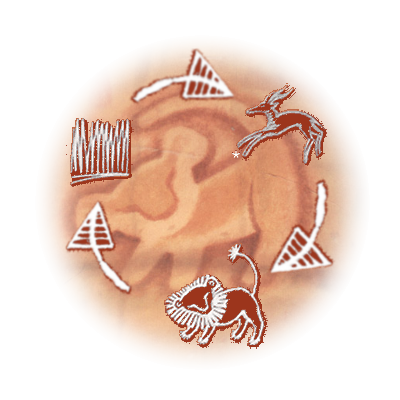
\includegraphics[scale=0.69]{images/circleEdited.png}\\
\bigskip
\LARGE{Patrick Misteli \& Ruben K{\"a}lin}

\bigskip

\bigskip

\bigskip

\bigskip

\bigskip

\bigskip

Zurich\\
May 2014\\

\end{center}



\newpage

%%%%%%%%%%%%%%%%%%%%%%%%%%%%%%%%%%%%%%%%%%%%%%%%%

\newpage
\section*{Agreement for free-download}
\bigskip


\bigskip


\large We hereby agree to make our source code for this project freely available for download from the web pages of the SOMS chair. Furthermore, we assure that all source code is written by ourselves and is not violating any copyright restrictions.

\begin{center}

\bigskip


\bigskip


\begin{tabular}{@{}p{3.3cm}@{}p{6cm}@{}@{}p{6cm}@{}}
\begin{minipage}{3cm}

\end{minipage}
&
\begin{minipage}{6cm}
\vspace{2mm} \large Patrick Misteli

 \vspace{\baselineskip}

\end{minipage}
&
\begin{minipage}{6cm}

\large Ruben K{\"a}lin

\end{minipage}
\end{tabular}


\end{center}
\newpage

%%%%%%%%%%%%%%%%%%%%%%%%%%%%%%%%%%%%%%%



% IMPORTANT
% you MUST include the ETH declaration of originality here; it is available for download on the course website or at http://www.ethz.ch/faculty/exams/plagiarism/index_EN; it can be printed as pdf and should be filled out in handwriting


%%%%%%%%%% Table of content %%%%%%%%%%%%%%%%%

\tableofcontents

\newpage

%%%%%%%%%%%%%%%%%%%%%%%%%%%%%%%%%%%%%%%



\section{Abstract}
In the film "Lion King" from Disney the main character's father explains to his son the concept of what he calls "the circle of life" and how all animals in the food chain hierarchy are needed in order for every species to survive. He abstracts the concept by explaining that lions become grass after they die. This grass is eaten by the antelopes, which are again eaten by the lions to complete the circle. We wanted to see if this concept is sound and said three organisms are able to survive within cellular automaton simulation.

\section{Individual contributions}
Patrick was responsible for the model, the parameters and the implementation in Matlab thereof. Ruben polished single aspects of the simulation and was responsible for the performance of the algorithm. Furthermore Ruben was responsible for the inclusion of the Lotka Volterra equation and finding papers thereof.

\section{Introduction and Motivations}
%Question 1: Is it possible to create a stable system? Yes
%Question 2: Is it possible for the system to remain stable if we were to remove one of the organisms? NO, Lotka Volterra: YES
Having a clear food chain hierarchy defined by the given "circle of life", we were not only interested in whether it is possible to create a stable system, but also which parameters effect the system in what way. Changing a minor parameter, for example how fast animals are able to reproduce or how hungry they are could have a major effect on the balance. Is it possible for the system to remain stable if we were to remove one of the organisms? To the end of the mentioned film "Lion King" the balance is destroyed when the lions start disrespecting the circle of life by overfeeding. Our model should be able to reproduce this effect when making the simulated lions "very hungry".
%Question 3: Do the two models, the Lotka-Volterra model and our model match in the sense, that they show the same simulation results? YES, except when removing lions
A very popular way of modeling the dynamics in populations is to use the Lotka-Volterra equations, \cite{lotkaVolterra}. Since we are using this model as a reference to our model, one of our fundamental research questions is whether it is possible to adjust our model to show similar results as the Lotka-Volterra model.

\section{Description of the Model}
\subsection{States}
Starting with Conway's Game of Life \cite{gameOfLife} a cell should not only have two states (active or inactive) it should now have the following four states representing all organisms:

\begin{description}
  \item[Nothing or Inactive (Black)] \hfill \\
	This represents a dead land cell where no living organism is located
  \item[Grass (Green)] \hfill \\
	This represents a living grass organism
  \item[Antelope (Brown)]  \hfill \\
	This represents a living antelope organism
  \item[Lion (Red)] 
   \hfill \\This represents a living lion organism
\end{description}

\subsection{Attributes}
Furthermore each of the four cell types must have parameterizable attributes in order for the extended rules to work. 
Table \ref{tab:Properties} lists all attributes and describes their meaning.

\begin{table}[htbp]
\newcounter{attCounter}
\setcounter{attCounter}{0}
\centering
\begin{tabular}{l|p{10.3cm}}
Name [Value Range]& Description\\
\hline
\hline
\addtocounter{attCounter}{1}
\arabic{attCounter}. Type \{1,2,3,4\}& The number between 1 and 4 represents "Nothing", "Grass", "Antelope" and "Lion" respectively  \\ 
\hline 
\addtocounter{attCounter}{1}
\arabic{attCounter}. PreyType \{1,2,3,4\} & Type of the organism which the current organism eats \\ 
\hline 
\addtocounter{attCounter}{1}
\arabic{attCounter}. Becomes \{1,2,3,4\}& Type to become after a natural death (Dying of age or hunger) \\ 
\hline 
\addtocounter{attCounter}{1}
\arabic{attCounter}. FoodDigest [0,inf]& Amount of food that is digested in one time-step\\ 
\hline 
\addtocounter{attCounter}{1}
\arabic{attCounter}. Stomach [0,inf]& Amount of food currently in organism. This decreases with each time-step (by the number defined in FoodDigest) and increases when the organism found food\\ 
\hline 
\addtocounter{attCounter}{1}
\arabic{attCounter}. MaxStomach [0,inf]& Maximal amount of food an organism will eat. Organism will only eat if its stomach is below this number. A high number will cause the organism to eat anything it finds causing overfeeding while a low number will cause the organism to live on a diet \\ 
\hline 
\addtocounter{attCounter}{1}
\arabic{attCounter}. DeathProb [0,1]& The probability of dying by age at the end of a time-step. Other death causes are discussed in section \ref{tab:deathCauses} \\ 
\hline 
\addtocounter{attCounter}{1}
\arabic{attCounter}. Fatness [0,inf]& The number of predators that can be fed eating this organism (Note: as soon as one predator takes a bite the current organism will become Nothing at the end of the time-step)\\ 
\hline 
\addtocounter{attCounter}{1}
\arabic{attCounter}. Alive \{0,1\}& 1 if alive, 0 if a predator has bitten this organism\\
\hline 
\addtocounter{attCounter}{1}
\arabic{attCounter}. MinStomachRep [0,inf]& Minimal value of Stomach needed to reproduce (Reproduction explained in section \ref{tab:reproduction}) \\
\hline 
\addtocounter{attCounter}{1}
\arabic{attCounter}. ReproductionProb [0,1]& Probability to reproduce when allowed (Reproduction explained in section \ref{tab:reproduction})\\
\hline 
\addtocounter{attCounter}{1}
\arabic{attCounter}. IsOffspring \{0,1\}& 1 if newborn, 0 if adult\\
\end{tabular}
\caption{A description of all attributes that define an organism.}
\label{tab:Properties}
\end{table}

\subsection{Protocol per Timestep}
Once we have generated an initial map with random cells we start the time process. This means for an unlimited amount of time steps every cell gets called in random order and completes the protocol. This protocol is very similar to the rules in Conway's Game of Life but has various extensions in order to simulate the behavior of nature. The following is a detailed description of what each cell processes in one time-step. Figure \ref{fig:protocol} visualizes this process further.

\thispagestyle{empty}
\begin{figure}[p]
\centering
\vspace*{-2cm}
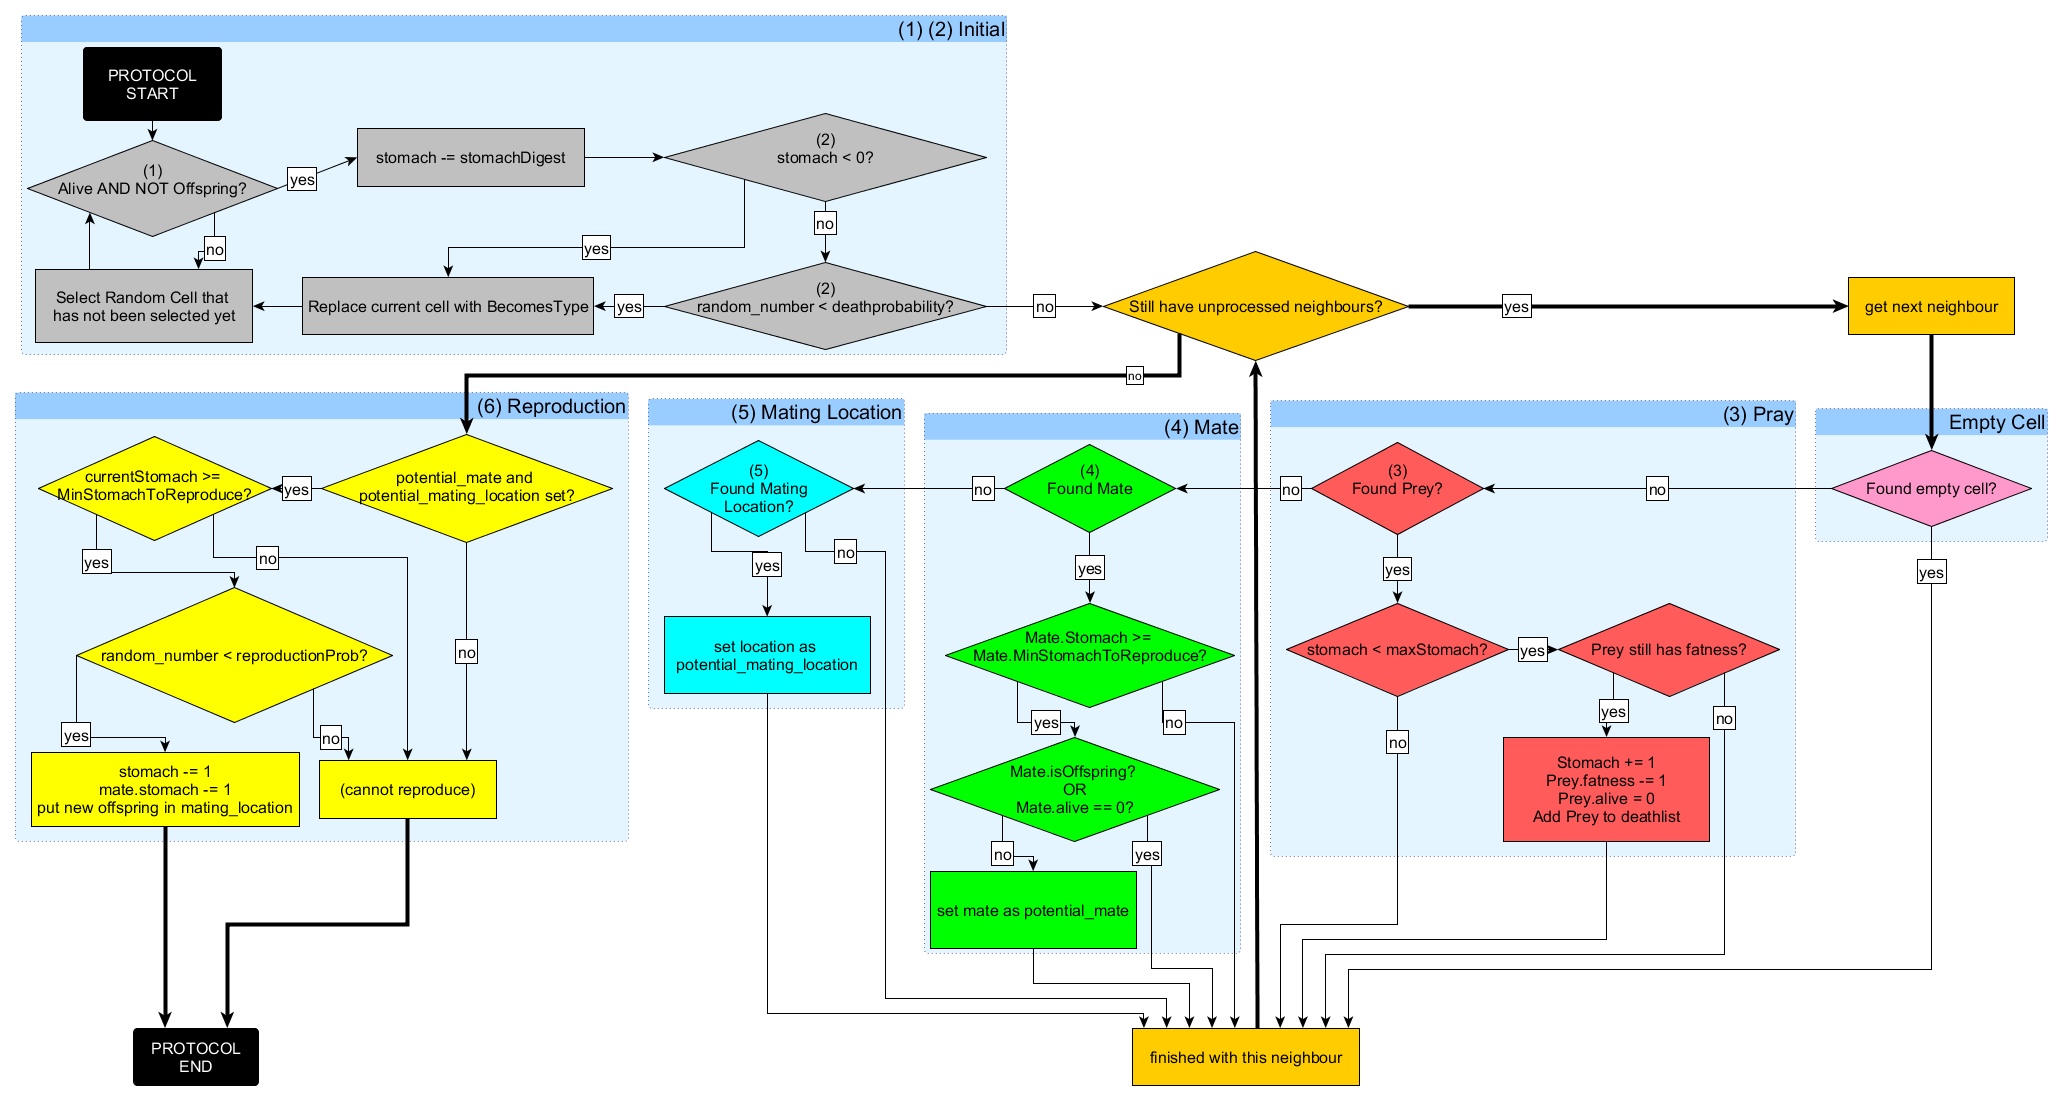
\includegraphics[angle=90,scale=0.34]{DayProtocol.png}
\caption{Protocol for each time-step}
\label{fig:protocol}
\end{figure}


\newcounter{protocolCounter}
\setcounter{protocolCounter}{1}
\subsubsection{(\arabic{protocolCounter}) Initial check} 
Here we check whether the {\it Alive} attribute is still set to 1. If it is set to 0 it means at least one predator cell has taken a bite of the current organism in this time-step.  This corresponds to a predator killing its prey in nature. If the the current cell is declared as dead it cannot (naturally) do anything anymore. We thus skip the protocol from here on and initiate the protocol on a next cell. We do not remove the organism yet, since more predators may be within the neighborhood and feed on this organism.
\\We furthermore check whether the current cell is an offspring ({\it IsOffspring} $== 1$). This would mean 2 other cells of the same type have generated this cell in this time-step. A newly born cell is also unable to do anything and we therefore would skip the rest of the protocol from here on. In nature, a newly born animal is able to neither reproduce nor hunt on directly. We are aware that there are animals who are able to hunt directly "out of the shell" (such as crocodiles), but we are dealing with antelopes and lions in our simulation which do not posses such skills. In addition, this attribute prevents a chain reaction of organisms generating many generations of children in one step. For example: Two lions produce an offspring in an empty field next to them. The offspring could then be able to reproduce with one of its parents in a cell next to it. Hyperpolating this will result in a chain of newborn lions in only one time-step.

\addtocounter{protocolCounter}{1}
\subsubsection{(\arabic{protocolCounter}) Livability Check} 
We now subtract what we have in the stomach by the number defined in the digestion attribute. If this causes a negative number in the stomach the organism has died of hunger and is instantly replaced by the type defined in its "Becomes" attribute. Furthermore we generate a random number. If this number is smaller than the death probability attribute the organism has died of age. As having died of hunger the organism is instantly replaced by the type defined in its "Becomes" attribute.\\
If the organism has died we skip the rest of the protocol and move on to the next cell. If the organism is still alive we can move on to the next protocol step. From here on we consider the neighborhood around the cell and act accordingly. The neighborhood is further described in section \ref{sec:neighbourhood}.
\addtocounter{protocolCounter}{1}
\subsubsection{(\arabic{protocolCounter}) Found Prey}
If we find an organism within the neighborhood who's type matches the type which was set in the current cell's PreyType attribute we have found food. We check whether out pray still has {\it fatness} left by checking its fatness attribute. An organism can only feed a fixed amount of predators. This amount is stored in the fatness attribute. The attribute is used to limit the number of predators who can eat this organism. Setting it to 1 means only one predator is able to feed himself before the prey becomes inedible. This corresponds to antelopes or grass only being able to fill the stomach of a certain amount of lions or antelopes respectively.\\
If the organism we encountered still has fatness larger than 0 we make sure the {\it Alive} attribute is set to 0 to incapacitate it. If this was not the case before we furthermore add the organism to a "deathlist". This list is used to keep track of all eaten organisms and after each time-step all organisms on the deathlist are removed (i.e become Nothing). 

\addtocounter{protocolCounter}{1}
\subsubsection{(\arabic{protocolCounter}) Found Mate}
If we find an organism who's type is equal to the current organisms type we check if it is possible to mate with it. This is done by ensuring the neighbor organism is alive ({\it Alive} attribute == 1) and that it has a high enough {\it Stomach} attribute in order to reproduce. I.e. the {\it Stomach} attribute must be equal or higher to the amount of the {\it MinStomachRep} attribute. Furthermore we ensure that the neighboring organism is not an offspring since a freshly born organism is unable to reproduce. Again, we are aware that there exist animals that are able to reproduce within the first day they are born (i.e. a mayfly XXXXCITEXXXX), but Antelopes and lions are not amongst those. If all these conditions are met the neighboring animal is set as a potential mate. An organism can only have one potential mate per timestep in order to keep a realistic reproduction rate.

\addtocounter{protocolCounter}{1}
\subsubsection{(\arabic{protocolCounter}) Found Mating Location}
If we find either a Grass or a Nothing cell in the surrounding neighborhood we mark it as a potential mating location. A Nothing cell receives higher priority in order not to replace potential food for the antelopes. 

\addtocounter{protocolCounter}{1}
\subsubsection{(\arabic{protocolCounter}) Reproduce}
\label{tab:reproduction}
Once we have processed all the cells in the neighborhood we now survey the outcome of the mating situation. If there we have a potential mate and a potential mating location we can continue with the final mating protocol. This is done by checking if the current organism's {\it Stomach} attribute is equal or higher than the amount of its {\it MinStomachRep} attribute. If this is also the case it means there is a potential mate who is enough fed, a cell within the neighborhood that can be replaced by an offspring, and the current organism is fed enough to reproduce. For a final test we generate a random number between 0 and 1. Reproduction is only possible if this random number is smaller than the {\it ReproductionProbability} attribute of the organism type. This simulates natures success rate of giving birth. Having a reproduction probability of 1 would result in 100 $\%$ success rate given the previous conditions are met. When the two organisms successfully reproduce the stomach of the offspring is set to the average of its parents plus 1. This reflects natures way of disabling two underfed parents to reproduce a well-fed child and therefore creating already eaten food. In addition the two parents both lose 1 stomach point in order to keep reproduction to a limit. This should simulate the increase of life difficulty of an organism once it has produced an offspring. Reproduction is natural, but it also hinders the parent's flexibility in life. Subtracting one stomach point enforces this concept, since the organism must now work harder (eat more) in order to stay alive.

\subsection{Neighbourhood}
\label{sec:neighbourhood}
As in game of life we inspect our neighborhood, see what kind of cells we find and act accordingly. 
We started off with the standard Moore-neighborhood and started testing the results of extending this neighborhood. This extension allows an organism to "see" further in the map and therefore not only eat more but reproduce with organism further away. Effects of this are discussed in section \ref{sec:DiscNeighbourhood}

\subsection{Death Causes}
In our model there are multiple ways a single organism can cease to exist. Depending on the cause the resulting cell differs too. Table \ref{tab:deathCauses} shows all possible death causes.
\begin{table}[htbp]
\centering
\begin{tabular}{l|p{11cm}}
Death Cause & Description \\ 
\hline 
\hline 
Age & At each time-step a random number between 0 and 1 is generated. If this number is smaller than the specified death probability the organism dies of age and the cell is turned into the type that is set in its {\it Becomes} attribute\\ 
\hline 
Hunger & When an organism's stomach reaches a negative number it dies of hunger and the cell is turned into the type that is set in its {\it Becomes} attribute\\ 
\hline 
Eaten & An organism can be eaten by its predator (or multiple predators in one time-step). If this is the case the cell becomes Nothing after the time-step is completed. We chose not to let the cell become the type that is set in its {\it Becomes} attribute because after being eaten an organism mainly resides in the stomach of its predator and does not contribute to the outside land anymore\\  
\end{tabular}
\caption{All death causes considered in our model.}
\label{tab:deathCauses}
\end{table}

\subsection{Known limits}
\label{sec:knownLimits}
Our model has certain limits due to abstraction of the concept. One major limit is the inability to move. In nature a herd of antelopes would escape the danger if detected. Since our organisms are unable switch places with another cell, the only way to move is by producing an offspring in a cell within the neighborhood. This of course requires a second organism of the same type. Thus, a single organism is unable to move while multiple organisms may create the illusion of moving. This does not differ much from Conway's Game of Life, where cells are also unable to move but patterns (such as a "glider", \cite{gameOfLife}) create the visual illusion that it is moving across the land.
\section{Implementation}
We used Matlab to create our simulation and an X-by-Y-by-12 sized matrix to store the data where X and Y correspond to the size of the map (Discussion about map sizes in section \ref{sec:DiscMapSize}. Having a 3d matrix allowed us to keep multiple attributes for each cell. Each layer of the 3d Matrix corresponds to one of the 12 attributes. For visual representation we used the following four subplots:
\begin{itemize}
\item A color coded 2d matrix of the current land. This was obtained by taking the matrix at level 1 of the 3d matrix, which shows the type of organism for each location on the land
\item A stacked bar plot to show the amount of deaths for each organism and the cause thereof.
\item  A second stacked bar plot showing the previous stacked bar plot with normalized numbers. This gives a better view of the percentages of each death cause for each organism. 
\item A line plot with a line for each of the 3 organisms (Grass, Antelope, Lion). The x-axis represents the time where the unit is "timestep" and the y-axis represents the quantity of the organism. This graph shows the current population on the land.
\end{itemize}
The final plot is shown in figure \ref{fig:plotScreenshot}.\\
In order to disable an organism to be cornered by its predator we implemented the map with a wraparound, allowing an organism on the edge to reproduce or eat to/from a cell on the other side of the land. 
\begin{figure}
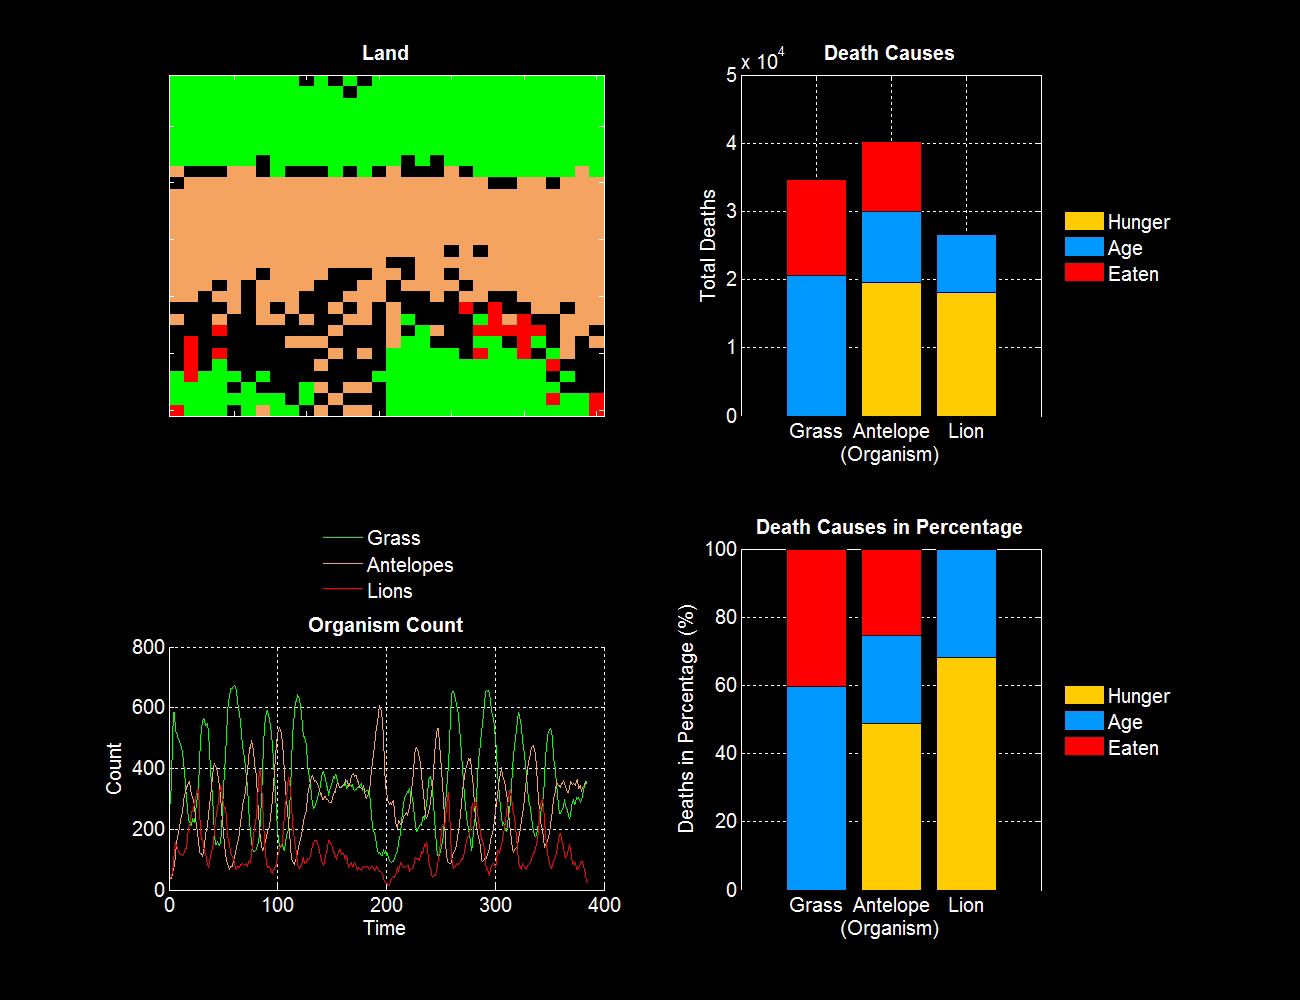
\includegraphics[scale=0.35]{plotScreenshot.png}
\caption{Four subplots}
\label{fig:plotScreenshot}
\end{figure}

\section{Lotka Volterra}
The population of different organisms has been thoroughly studied. A.J. Lotka and V. Volterra found formulas describing the population number of two species, \cite{lotka}, \cite{volterra}. One species is a predator and the other species is the prey. A large number of predators results in a decrease of prey organisms and a small number of predators allows prey organisms to increase in number. On the other hand, the predators are fed by the prey, so predators can only flourish when there are enough prey organisms to eat. When the number of prey organism becomes too little, predators die of hunger. These rules are reflected in the formulas of Lotka and Volterra, \cite{lotkaVolterra} which show the dynamics of the population.\\

\begin{equation}
\begin{split}
\frac{dx}{dt} = ax-bxy \\ 
\frac{dy}{dt} = cxy-dy
\end{split}
\end{equation}
The reasoning about the population count of organisms has been extended to three species, \cite{lotkaVolterraThreeSpecies} forming a food chain. In the model, organisms Z are predators of organisms Y and organisms Y prey on organisms X. Therefore, compared to the two species situation, the population count of organism Y now additionally depends on the number predators (organisms Z).
\begin{equation}
\begin{split}
\frac{dx}{dt} = ax-bxy \\ 
\frac{dy}{dt} = -cy+dxy-eyz \\ 
\frac{dz}{dt} = -fz+gyz
\end{split}
\end{equation}
The resulting curves can be parametrized by the initial population counts START_X, START_Y, and START_Z as well as the six constants a,b,c,d,e,f, and g as shown in Table \ref{tab:LotkaVolterraParameters}.
\begin{table}[htbp]
\centering
\begin{tabular}{l|l}
Parameter & Description \\ 
\hline 
\hline 
START_X & the initial number of organisms X
\hline
START_Y & the initial number of organisms Y
\hline
START_Z & the initial number of organisms Z
\hline
a & reproduction rate of organisms X\\ 
\hline 
b & disadvantage of organisms X of being hunted\\ 
\hline 
c & vulnerability of organisms Y to overpopulation\\  
\hline 
d & advantage of organisms Y of hunting\\
\hline 
e & disadvantage of organisms Y of being hunted\\
\hline 
f & vulnerability of organisms Z to overpopulation\\
\hline 
g & advantage of organisms Z of hunting\\
\end{tabular}
\caption{The semantic meaning of the different constants.}
\label{tab:LotkaVolterraParameters}
\end{table}
This model could be further generalized in a similar manner to model $n$ organisms. The behaviour of the population curves highly depends on the choice of variables and is thoroughly studied in \cite{lotkaVolterraThreeSpecies}. The variable assignment $a=b=c=d=e=f=g=1$ and with the initial populations $START_X= 0.5,START_Y = 1, START_Z=2$ results in the oscillating population count curves shown in Figure \ref{fig:LotkaVolterraThreeAllOnes}. 

\begin{figure}
\centering
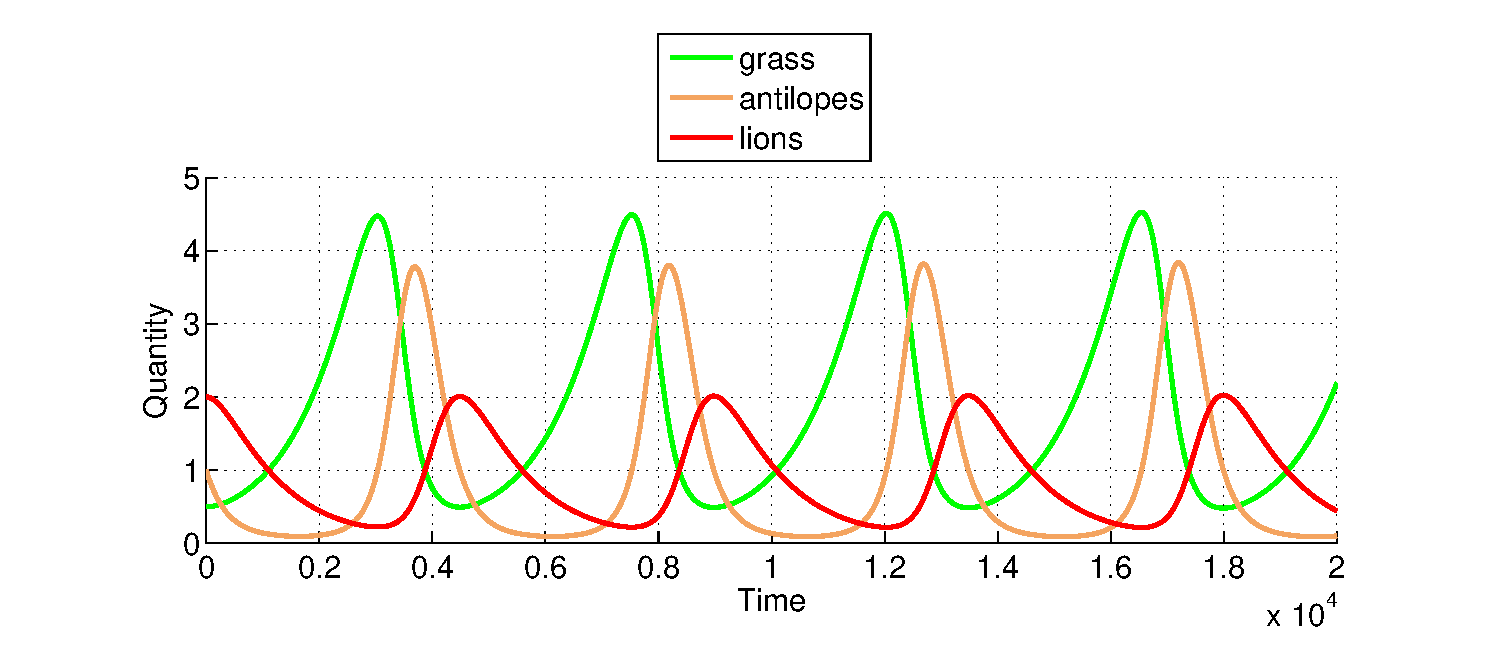
\includegraphics[scale=0.65]{LotkaVolterraThreeAllOnes}
\caption{Lotka-Volterra equations for $a=b=c=d=e=f=g=1,start_X=0,5, start_Y=1,$ and $start_Z=2$.}
\label{fig:LotkaVolterraThreeAllOnes}
\end{figure}

\section{Simulation Results and Discussion}
Running multiple simulations and adjusting the parameters and initial map there were several dependencies we discovered. Additionally we compared the population results obtained form the simulation with the Lotka-Volterra population curves for three species, \cite{lotkaVolterraThreeSpecies}. 

\subsection{Chosen Parameters}
A possibility of a simple parameter combination that produces a stable or oscillating population is given in table \ref{tab:ChosenParameters}.
The death probability was calculated using the helper function $deathProb(a) = 1-(\frac{a}{a+1})$ which takes input $a$ = average life expectancy and outputs the corresponding death probability.\\
We have decided NOT to let antelopes become grass when they die of age or hunger but rather become nothing. The reason for this is the dedication to a {\it Circle} of life. Antelopes get eaten by lions which become grass after they die which can then again be eaten by the antelopes. If antelopes were to become grass too after passing away there would be an additional arrow from antelope to grass. For the purpose of our model we decided against this addition. For simplicity we have left the minimum stomach to reproduce at 0, which means an organism will always be fed enough to reproduce.

\begin{table}[htbp]
\centering
\begin{tabular}{l|l|l|l|l}
\newcounter{attCounter2}
\setcounter{attCounter2}{0}
Attribute Type & Nothing & Grass & Antelope & Lion\\
\hline
\hline
\addtocounter{attCounter2}{1}
\arabic{attCounter2}. Type \{1,2,3,4\} & 1 & 2 & 3 & 4\\
\hline 
\addtocounter{attCounter2}{1}
\arabic{attCounter2}. PreyType \{1,2,3,4\} & -1 & -1 & 1 & 2\\ 
\hline 
\addtocounter{attCounter2}{1}
\arabic{attCounter2}. Becomes \{1,2,3,4\} & 0 & 0& 0 & 1\\ 
\hline 
\addtocounter{attCounter2}{1}
\arabic{attCounter2}. FoodDigest [0,inf]&0 & 0 & $\frac{1}{2}$ & 1 \\ 
\hline 
\addtocounter{attCounter2}{1}
\arabic{attCounter2}. Stomach [0,inf]& $\infty$ & $\infty$ & 10 & 10\\ 
\hline 
\addtocounter{attCounter2}{1}
\arabic{attCounter2}. MaxStomach [0,inf]& 0 & 0 & 10 & 10 \\ 
\hline 
\addtocounter{attCounter2}{1}
\arabic{attCounter2}. DeathProb [0,1]& $\infty$ & $\frac{1}{6}$ & $\frac{1}{10}$ & $\frac{1}{11}$\\ 
\hline 
\addtocounter{attCounter2}{1}
\arabic{attCounter2}. Fatness [0,inf]& 0 & 8 & 8 & 0\\ 
\hline 
\addtocounter{attCounter2}{1}
\arabic{attCounter2}. Alive \{0,1\}& 0 & 1 & 1 & 1\\
\hline 
\addtocounter{attCounter2}{1}
\arabic{attCounter2}. MinStomachRep [0,inf]& $\infty$ & 0 & 0 & 0\\
\hline 
\addtocounter{attCounter2}{1}
\arabic{attCounter2}. ReproductionProb [0,1]& 0 & 0.7 & 1 & 1 \\
\hline 
\addtocounter{attCounter2}{1}
\arabic{attCounter2}. IsOffspring \{0,1\}& 1 & 1 & 1 & 1\\
\end{tabular}
\caption{The chosen attributes for each organism.}
\label{tab:ChosenParameters}
\end{table}

\begin{table}[htbp]
\centering
\begin{tabular}{l|l|l|l|l}
Attribute Type & Nothing & Grass & Antelope & Lion\\
\hline
\hline
4. FoodDigest [0,inf]&0 & 0 & $\frac{1}{5}$ & $\frac{1}{5}$ \\ 
\hline 
5. Stomach [0,inf]& $\infty$ & $\infty$ & 2 & 2\\ 
\hline 
6. MaxStomach [0,inf]& 0 & 0 & 2 & 2 \\ 
\hline 
8. Fatness [0,inf]& 0 & 2 & 8 & 0\\ 
\hline 
10. MinStomachRep [0,inf]& $\infty$ & 0 & 1 & 1\\
\hline 
11. ReproductionProb [0,1]& 0 & 0.7 & 1 & 0.6 \\
\end{tabular}
\caption{The changed attributes from table \ref{tab:ChosenParameters} to work with a larger neighborhood}
\label{tab:NewParam}
\end{table}

\subsection{General Observations}
Our simulation is based on a set of inherently local rules. Two organisms only influence each other when both are in each others neighborbood. Therefore, the fastest possible propagation speed is one times the radius of the neighborhood per time-step. However, structures larger than one neighborhood can emerge over time when the influence spreads across the land. These macro phenomena seem to obey their own set of rules even if they are only the interaction between many cells. 
%Outline
In this section we introduce the patterns encountered during the simulations and explain why they naturally emerge.

\subsubsection{Oscillating or Stable population}
There are two types of population variation. A stable population is one where all organisms remain their numbers. It is important to note that organisms still reproduce and pass away, but the rate of reproduction and dying are almost equal at every time-step.\\
The second type of population we discovered was an oscillating population. Here the ratio from death rate to birthrate oscillates from one side to the other. Populations tend to oscillate because the different species depend on each other. Lions need to eat antelopes, antelopes need to eat grass and grass needs to have space to grow or be created by deaths of lions. At some point the grass population starts to grow as there are not enough antelopes to eat them. The more grass there is the better for the antelopes because they can feed themselves and their offspring. This results a decrease of grass organisms and an increase in antelopes. An increase in antelopes means a better life set up for lions since now they are able to feed themselves and their offspring. This results in an increase of lions and decrease of antelopes. Having no food left, the lions start dying and becoming grass. This results an increase of grass since not only the lions generate it but there are little antelopes left to prevent the growth of the grass population. More grass and less lions is a good life set up for antelopes to start growing again and so forth.\\
This oscillation can have different sizes. A large size of oscillation means animals go from overpopulation to almost extinction. A very small oscillation could be regarded as almost stable. if the oscillation is too large one organism takes over and wipes the entire land. Reasons for this are discussed in section \ref{sec:DiscNeighbourhood} and section \ref{sec:DiscMapSize}.\\
In addition it is possible that an oscillating map will find an almost stable state, while an almost stable state may start oscillating again. Figure \ref{fig:plotScreenshot} shows an oscillating state between the time-steps 0-120. An almost stable state follows till time-step 180 after which the oscillation is re-initiated. 


\subsubsection{Patterns}
\label{sec:patterns}
As in Conway's Game of Life there are certain patterns that appear when we start with a randomized land. This is the case even though the selection of each cell and the selection of its corresponding neighbor happens in random order.  At first there is a strong oscillation until small groups (or "herds") have formed. At the beginning the location is not a big factor since all animals are placed randomly on the map. Thus the behavior is much like the one described by the Lotka-Volterra equation. After a while organisms that were near at the beginning start forming a herd, while lonely organisms die out because of the incapability to reproduce on their own. 
Two patterns with known consequences were observed
\begin{itemize}
\item {\bf Chased Antelope Herd:} An antelope herd is formed as described above. A lion herd can "dock" against one side of this herd. This results in antelopes only being able to reproduce on one side of the herd where on the other side of the herd the lions eat the antelopes and produce new offsprings in the now empty cells. If an antelope would produce an offspring in a cell of an eaten antelope it would probably get eaten in the next timestep by a neighboring lion. The side of the lion herd that is not facing the antelope herd die out because of lack of food. This produces two adjacent herds where one side is well nourished and can reproduce (i.e. move) while the other side has no food and/or predators eating them. Figure \ref{fig:chasedAntelopesHerd} shows this pattern.
\item {\bf Lion Island:} A lion island is formed when a lion herd is surrounded by antelopes. This means the lions can reproduce in all directions and thus expand the herd quickly. Since the grass generated by passing away lions is surrounded by well-fed lions it is inaccessible for the antelopes (unlike the previous "chased antelope herd" pattern). In the extreme case this could lead to a wipeout of all animals. Figure \ref{fig:lionIsland0} demonstrates this effect. The antelopes start overfeeding while only two small lion herds remain. In Figure \ref{fig:lionIsland1} the lions are completely surrounded and start expanding. \ref{fig:lionIsland2} shows that the only grass on the map is guarded by a circle of lions and thus inaccessible for antelopes. Figure \ref{fig:lionIsland3} shows the consequence of this. The lions have evetually eaten all antelopes and are dying out because of hunger and age. The map size is important for this effect to wipe out the land. This is discussed in section \ref{sec:DiscMapSize}.
\end{itemize}

\begin{figure}
\centering
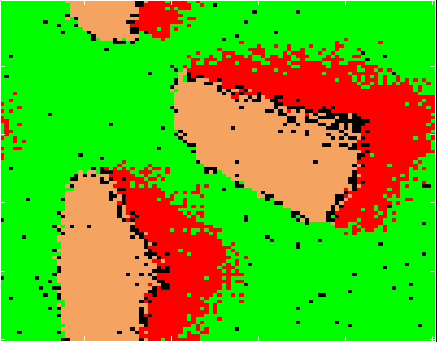
\includegraphics[scale=1]{chasedHerd}
\caption{Lions chasing a herd of antelopes.}
\label{fig:chasedAntelopesHerd}
\end{figure}

\begin{figure}
\centering
\subfloat[MISSING CAPTION]
{
\includegraphics[width=0.5\textwidth]{lionIsland0.png}\label{fig:lionIsland0}
}
\subfloat[A small group of lions surrounded by antelopes.]
{
\includegraphics[width=0.5\textwidth]{lionIsland1.png}\label{fig:lionIsland1}
}
\newline
\subfloat[Surrounded lions start expanding and prevent antelopes from reaching grass.]
{
\includegraphics[width=0.5\textwidth]{lionIsland2.png}\label{fig:lionIsland2}
}
\subfloat[Extinction of antelopes can result from surrounded lions.]
{
\includegraphics[width=0.5\textwidth]{lionIsland3.png}\label{fig:lionIsland3}
}
\caption{Various emerging patterns.}
\label{fig:circleOfLifePatterns}
\end{figure}

\subsubsection{Location Dependency}
\label{sec:DiscLocationDep}
The main difference between our model and the Lotka-Volterra equation is that Lotka-Volterra only takes into account the quantity of the population, but not the location thereof. In a land where antelopes and lions are separated too far away it is not possible for them to have any effect on each other. This was already mentioned in section \ref{sec:knownLimits}. In our simulation we experienced extinctions of a species simply because they were unable to reach its food source in time before dying of age or hunger. Species may not only be unable to reach food source but may also be unable to reach a potential mate, which makes reproduction impossible. When having one species gone extinct it is usually only a matter of time until another species will go extinct as well. This is further elucidated in section \ref{sec:DiscRemovalOfOne}.

\subsubsection{Random Selection vs Sequential Selection}
We have designed to randomly select a cell in one time-step to update while making sure that every cell gets updated exactly once per time-step. Furthermore the selection of the neighboring cell is also randomly selected from the defined neighborhood. In an initial attempt we had both selections running in sequential order. This caused certain patterns to always move to the top left since those cell are updated first. By being updated first they are able to feed first before the others get a chance. Furthermore if no empty cells are in the neighborhood, the first grass cell on the top left will always be selected to turn into an offspring. By making it random we make sure no predefined pattern and pattern-direction can occur due to the updating order.

\subsubsection{Map Size} %TODO: REVISE SECTION
\label{sec:DiscMapSize}
As mentioned in section \ref{sec:DiscLocationDep} the location and surrounding of each organism is vital for its survival. Thus the size of the land plays an important role. A smaller map enables a single organism to have everything in its neighborhood and act accordingly. This is especially "good" for lions since they will always have potential food in its neighborhood. A takeover by lions is therefore very likely in a small map unless the lions are tamed by adjusting their parameters to only eat very few antelopes.\\
Oscillations in a small land are difficult to achieve because not much freedom is allowed. As soon as one organism takes over it could mean the extinction for another one due to little space left and due to inability to escape its predator.\\
Having a larger land a Lion Island pattern (section \ref{sec:patterns}) does not guarantee the extinction of antelopes. The reason for this is that a herd of antelopes could exist with a distance great enough for the lions not to reach them. As soon as the lions run out of antelopes to eat they start dying of hunger and the protecting lion-circle around the grass is broken.

large oscillation 
Patterns remain the same (except if we change the neighborhood). Small map is more likely to fall apart. The size of "Wipeouts" is fixed. Wipeout = one organism takes over. The oscillations on small maps have a higher amplitude and thus, have a larger tendency to become unstable. On a large map multiple wipeouts can equalize each other.
in conclusion: larger maps lead to stable non-oscillating cycles with a good chance of all species surviving. 

In larger lands oscillating structures have a fixed size. Therefore, a larger land contains more oscillating structures that do not need to be in the same state because our model only considers local neighborhoods. The phase shift between the oscillating structures evens out the overall population counts. Therefore, the population curves for larger lands tend to stabilize close to an equilibrium whereas lands with a size small enough to fit only one or few oscillating structures show a clear oscillation. Lands that are too small to fit an oscillating structure show an extinction of a race or result in a complete wipeout.\\

Islands of Lions. Large Map results smaller probability of this happening.

\begin{figure}
\centering
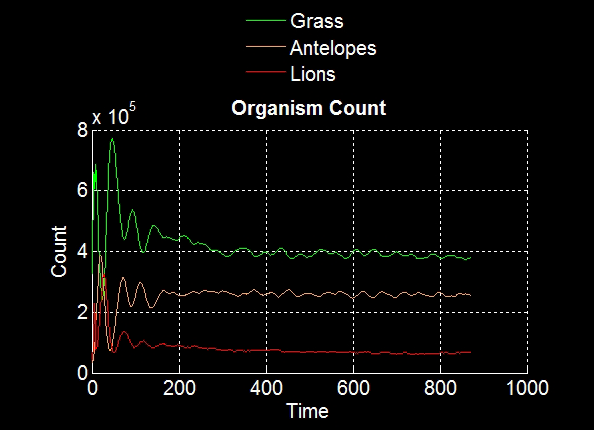
\includegraphics[scale=0.7]{circleOfLifeLargeLand}
\caption{Circle of life simulation with large land 1000x1000 cells.}
\label{fig:CircleOfLifeLarge}
\end{figure}

\subsubsection{Neighborhood Size}
\label{sec:DiscNeighbourhood}
In our model we have chosen the Moore neighborhood and extended it by adding one more field to the northern, eastern, southern and western neighbor, \cite{mooreNeighborhood}. The so produced neighborhood is known under the name of "Von Neumann neighborhood" with a manhatten distance of 2, \cite{vonNeumannNeighborhood}.  produces a 12-connected-neighborhood which seemed an optimal view depth for each organism with our chosen parameters. Decreasing this relates to a slightly blind organism. It cannot see the possible food or mate around it and will therefore die quicker of hunger without being able to reproduce before. Increasing this relates to giving each organism super-vision of the land. A predator is able to eat another cell further away. which means escaping of one species from its predator gets harder. The simulation with our chosen parameters showed that an organism who is able to see the next three neighbors (48-connected-neighborhood) already affects the oscillation of the population in a way where extinction of one species is almost guaranteed. This happens because with our parameters we allow an organism to eat until its stomach is full (MaxStomach = 10) and reproduce until its stomach is empty. Therefore, each organism is able to reproduce with up to 10 organisms that choose the observed organism as a mate in a single time-step. This may cause overpopulation and result in extinction (further explained in section \ref{sec:DiscRemovalOfOne}). However, on average an organism can still only actively initiate one reproduction per time-step. Adjusting the parameters to allow a stable population with a 48-connected-neighborhood is possible. The adjusted values are shown in table \ref{tab:NewParam}. We adapted the food digestion speed in order for animals to live longer without the need to feed. We also lowered the initial Stomach and MaxStomach to prevent lions and antelopes to overfeed. The fatness of grass was also lowered to only allow 2 antelopes to feed from one grass cell. Lastly the reproduction was adjusted by setting a higher minimum stomach and a lower reproduction probability in order to make producing offspring less likely and preventing an overpopulating of the land.\\
An interesting aspect of the new setup is that it does not work for a smaller neighborhood. The reproduction probability is already lowered and taking away 36 of the previously 48 possible mates and mating location makes it even less likely for an organism to reproduce. 

\subsubsection{Removal of one species}
\label{sec:DiscRemovalOfOne}
When our Model is started without any grass, then the population counts may still behaves the same as if grass was added at the beginning, because once a lion dies, it becomes grass. Therefore, the antelopes can potentially reach grass, survive and keep up the balance. However, since the antelopes need to go pass the lions to reach grass it is rather unlikely that lions and antelopes survive. The smaller the land is the smaller the probability that the land recovers from the initially strongly unbalanced situation.\\
When no antelopes are added in the beginning, all lions starve for sure, because thy cannot reach there prey. The grass population then fills the entire land and hits a hard limit because there are no more cells to populate. \\
If initially no lions are added to the land there are two different outcomes: Either the antelopes eat all the grass and then starve leaving an extinct land, or both species survive. The latter case is more probable in larger lands, whereas in smaller lands the species seldom survive.

We applied the same modified initial conditions to the Lotka-Volterra model and compared the result.
Removing one of the species impacts the population curves in the following way: Figures \ref{fig:removeAllGrass}, \ref{fig:removeAllAntelopes}, and \ref{fig:removeAllLions}. In the Lotka-Volterra model removing all grass unavoidably leads to the extinction of all organisms, because all antelopes starve and therefore, also all lions die of hunger.\\
When there are no antelopes, the food chain is broken and all the lions starve. The grass can flourish because it has no natural enemies. Additionally, the missing capacity limit enables the grass population to grow indefinitely.\\
Removing only the lions simply reduces the Lotka-Volterra model for three species to the model with only 2 species and thus, the population of the grass and of the antelopes could be self regulating and the curves might oscillate. However, because the Lotka-Volterra equations for three species require a different parameter setting to show an oscillating behaviour, only removing the lions and keeping the parameters set for three species results in the antelopes eating all the grass and then slowly starving.\\

For the our model the situation is different in some ways, because we consider locations and neighborhoods rather than only advancing based on pure population count. Additionally the size of our land is limited to a fixed number of cells. Therefore a indefinite population growth cannot occur in our model. The overall trends however match nicely between the two models.

\subsection{Overfeeding}

\subsection{Other}

\begin{table}[htbp]
\centering
\begin{tabular}{l|l}
Parameter & Value \\ 
\hline 
\hline
start\_X & 300\\
\hline
start\_Y & 30\\
\hline
start\_Z & 30\\
\hline
a & 0.2143\\ 
\hline 
b & 0.0014\\ 
\hline 
c & 0.0014\\  
\hline 
d & 7.1492e-04\\
\hline 
e & 0.0014\\
\hline 
f & 0.2143\\
\hline 
g & 0.0014\\
\end{tabular}
\caption{The choice of constant values for the comparison with the simulation results}
\label{tab:LotkaVolterraParametersFinal}
\end{table}

The graphical result of the Lotka-Volterra equations for these parameters is shown in Figure \ref{fig:LotkaVolterraThreeAdjusted}.

\begin{figure}
\centering
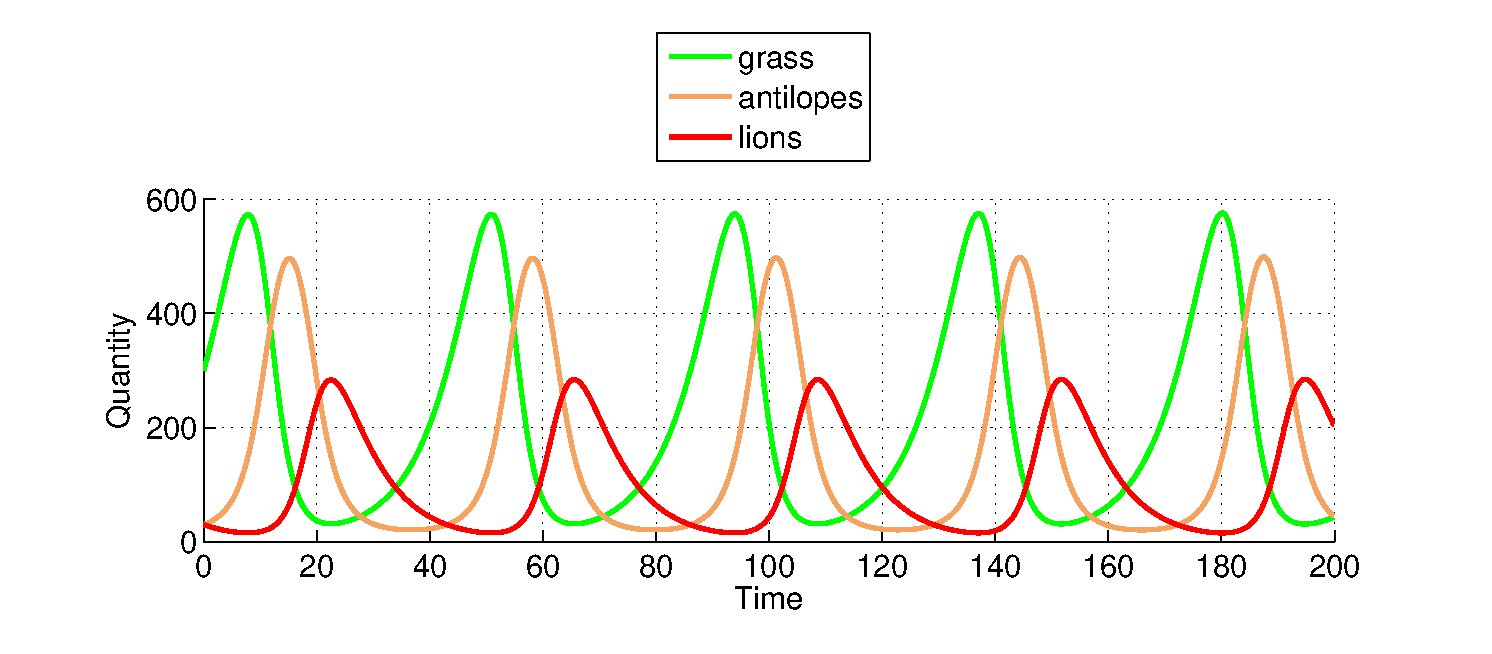
\includegraphics[scale=0.7]{LotkaVolterraThreeAdjusted}
\caption{Lotka-Volterra equations for the parameters as shown in Table \ref{tab:LotkaVolterraParametersFinal}.}
\label{fig:LotkaVolterraThreeAdjusted}
\end{figure}

\begin{figure}
\centering
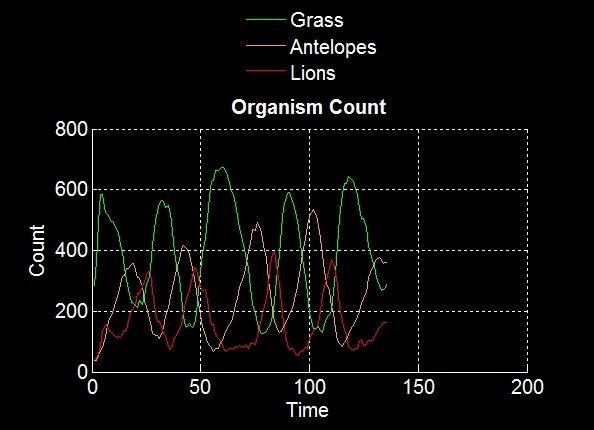
\includegraphics[width=0.8\textwidth]{circleOfLifeOscillating.png}
\caption{Circle of life simulation with oscillating behaviour.}
\label{fig:noGrass}
\end{figure}

\begin{figure}[p]
\centering
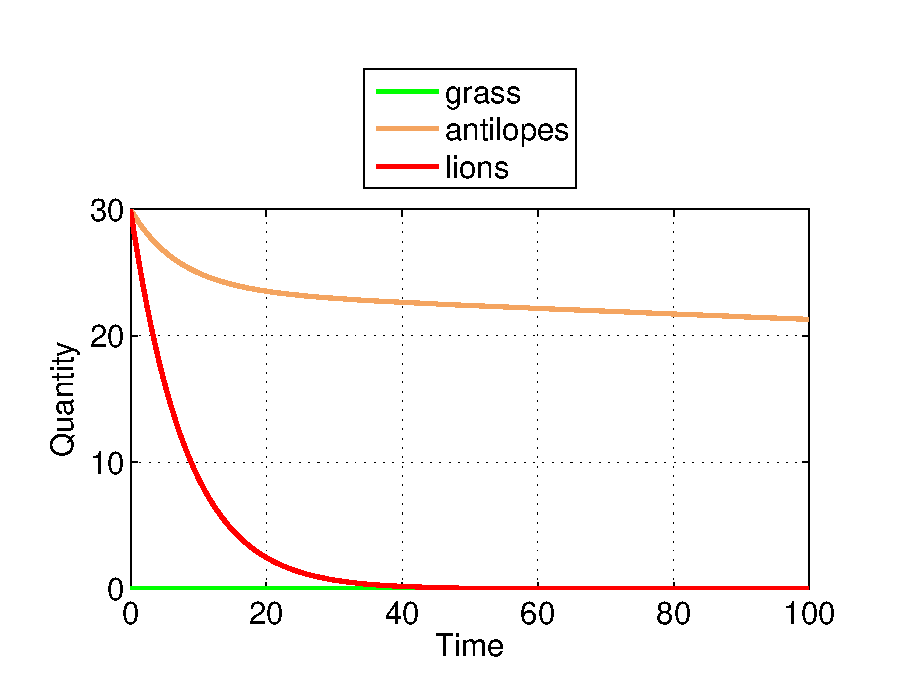
\includegraphics[width=0.7\textwidth]{LotkaVolterraNoGrass.eps}
\caption{Lotka Volterra equations, result of starting with zero grass.}
\label{fig:removeAllGrass}
\end{figure}

\begin{figure}
\centering
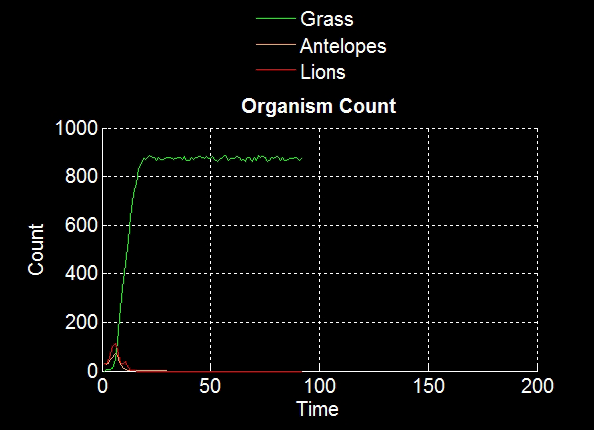
\includegraphics[width=0.8\textwidth]{noGrassOnlyCount.png}
\caption{Circle of Life simulation with initially no grass. Since dying lions}
\label{fig:noGrass}
\end{figure}

\begin{figure}
\centering
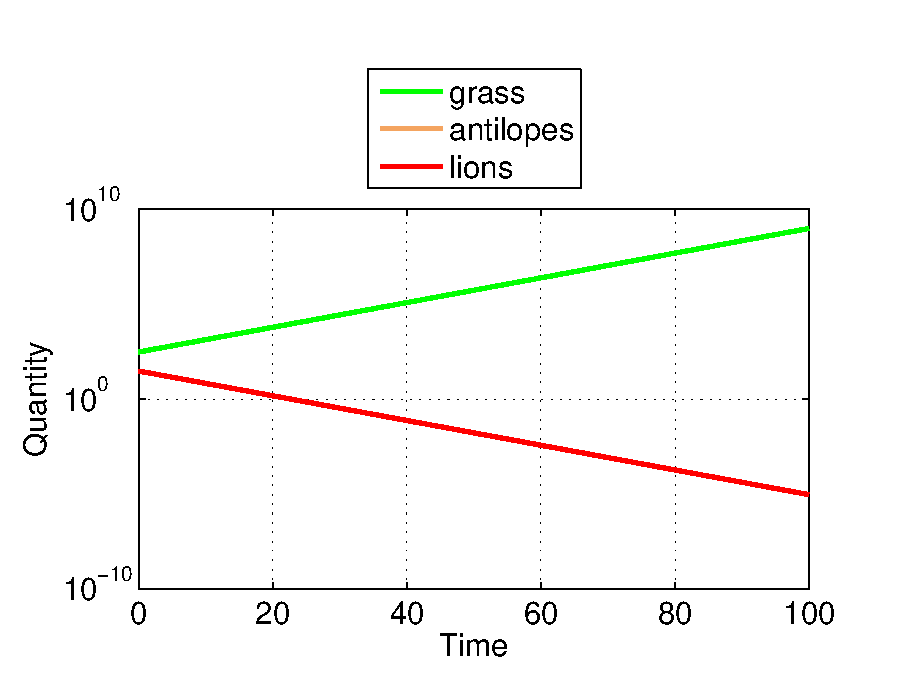
\includegraphics[width=0.7\textwidth]{LotkaVolterraNoAntelopes.eps}
\caption{Lotka Volterra equations, result of starting with zero antelopes.}
\label{fig:removeAllAntelopes}
\end{figure}

\begin{figure}
\centering
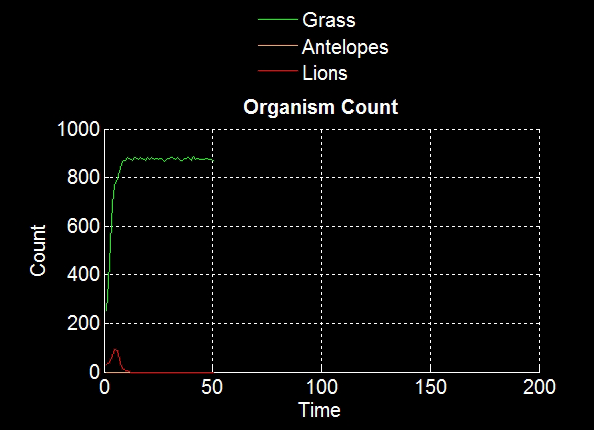
\includegraphics[width=0.7\textwidth]{noAntelopesOnlyCount.png}
\caption{Circle of Life simulation with initially no antelopes.}
\label{fig:noAntelopes}
\end{figure}

\begin{figure}
\centering
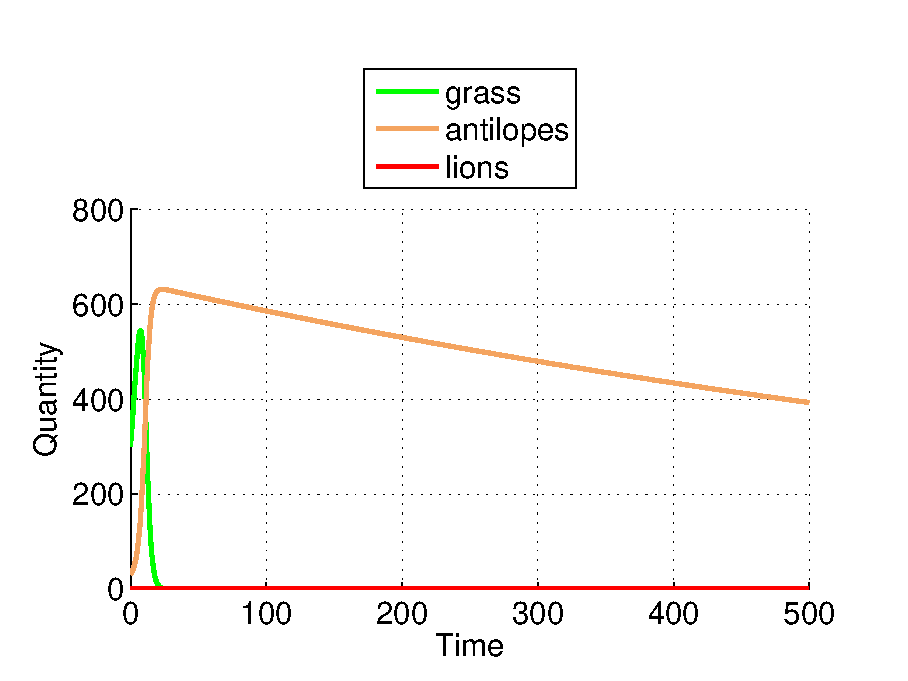
\includegraphics[width=0.7\textwidth]{LotkaVolterraNoLions.eps}
\caption{Lotka Volterra equations, result of starting with zero lions.}
\label{fig:removeAllLions}
\end{figure}

\begin{figure}
\centering
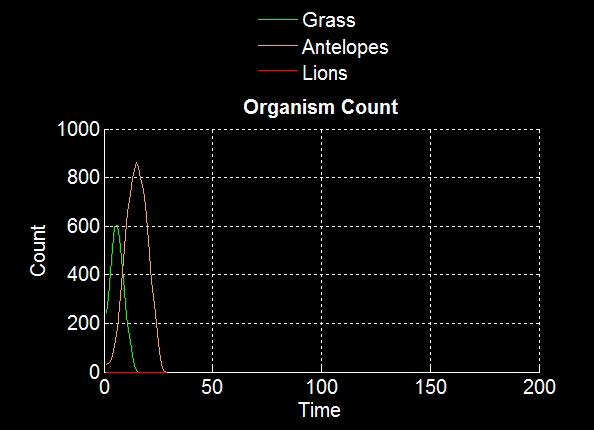
\includegraphics[width=0.8\textwidth]{noLionsOnlyCount.png}
\caption{Circle of Life simulation with initially no lions.}
\label{fig:noLions}
\end{figure}

\ifx
\begin{figure}
\centering
\subfloat[Removing grass]
{
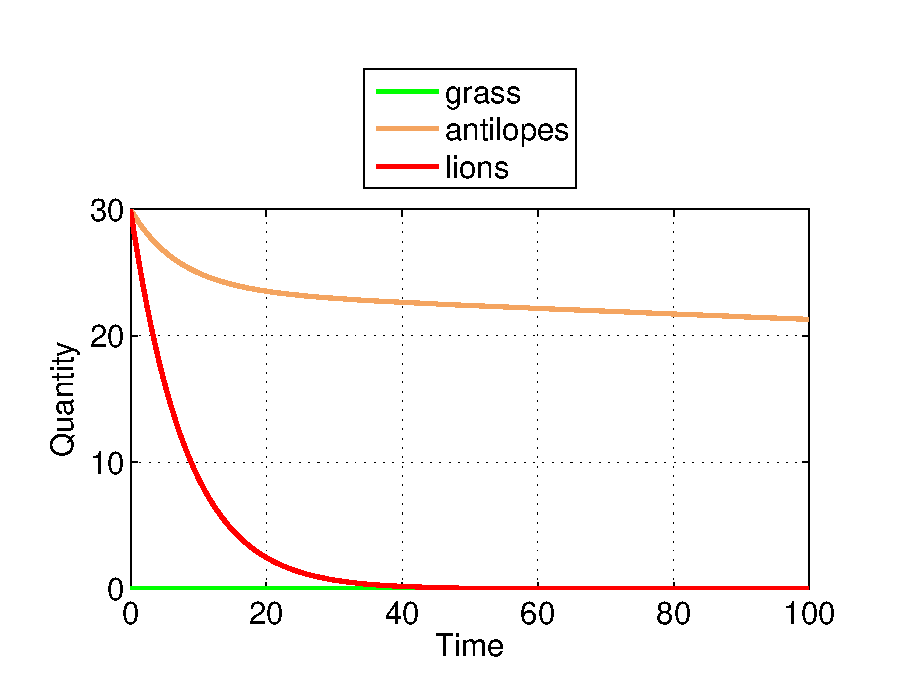
\includegraphics[width=0.9\textwidth]{LotkaVolterraNoGrass.eps}
}
\newline
\subfloat[removing antelopes]
{
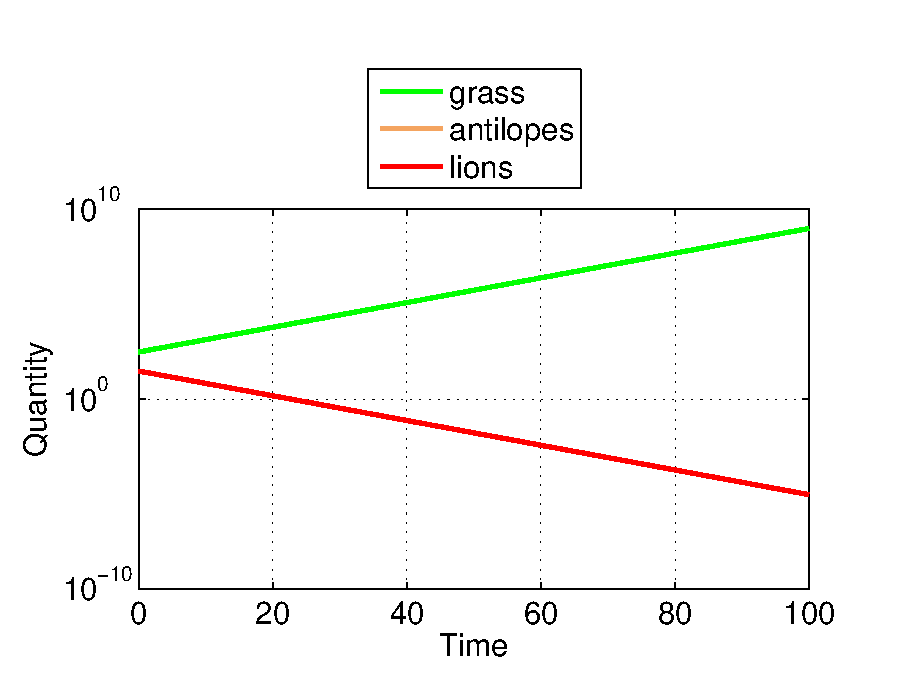
\includegraphics[width=0.9\textwidth]{LotkaVolterraNoAntelopes.eps}
}
\newline
\subfloat[removing antelopes]
{
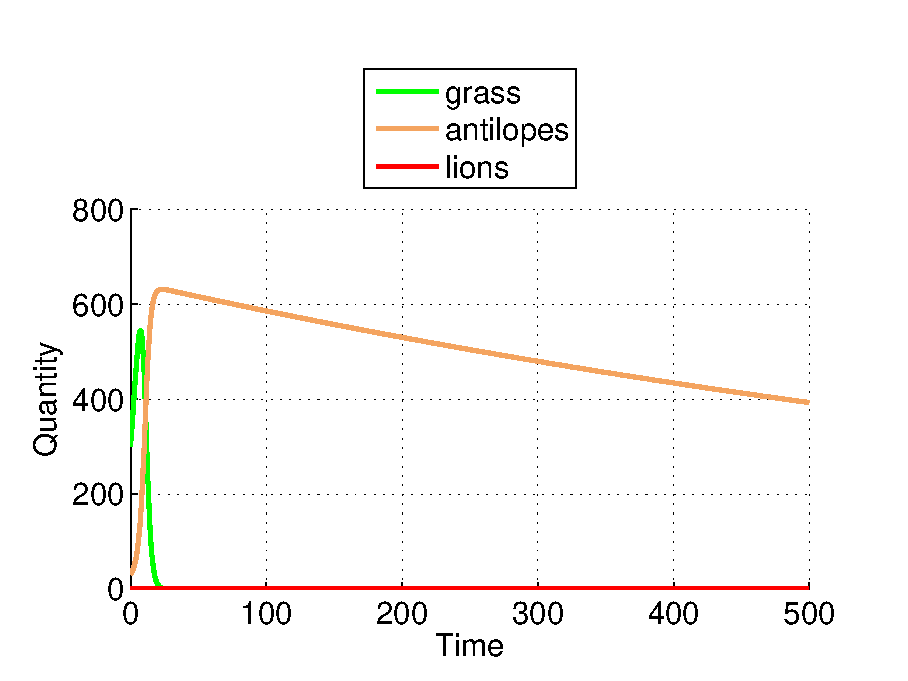
\includegraphics[width=0.9\textwidth]{LotkaVolterraNoLions.eps}
}
\caption{Result of removing all instances of one organism.}
\label{fig:removingOneOrganism}
\end{figure}
\fi


\section{Summary and Outlook}

Adjusting the parameters in the Lotka-Volterra formulas to the values shown in Table \ref{tab:LotkaVolterraParametersFinal} results in  population curves similar to the ones obtained from our simulation. Therefore, we conclude that our simulation models the habitat of organisms is somewhat consistent to the Lotka-Volterra equations for the situation that all three species are present.


Answer questions
Location of animals important. It is not taken into account by lotka-volterra.

Dependent of each other. 
Only antelopes and grass causes wipeout. with larger lands most of the time stable

 

\appendix

\section{Appendix}
The title image was taken from \cite{titleImage}.

\section{Code}
%the final source code goes here

\bibliographystyle{plain}
\bibliography{bibliography}
\addcontentsline{toc}{section}{Bibliography}

\end{document}  